
\section{ping/peek performance test 1}
\subsection{Purpose}
The purpose of this experiment is to measure the roundtrip time, latency, between a sensornode and a border gateway using ping and CCN peek commands. The results show which of these alternatives has the lowest latency, how much they differ and if there is a common pattern between them. It is also interesting to see how much time it takes for a sensor node to consume an CCN interest. From a more overview perspectrive, it is very important that the processing time of a CCN interest does not take to long time or to much resources and that it should be feasible for a sensor to deal with. If the computation time of returning data is to large, then CCN would be considered not suitable to be used for a IoT device. From here on, latency and round trip time is used interchangeably aswell as CCN peek and peek.

[Make the nice picture and write about why that picture is interesting. This could be something in the beginning of the result section, the arguments could be around it. Showing the roundtrip time and processing time.]

\begin{itemize}
    \item formulera purpose of this experiment, på en högre nivå, vad är det som motiverar varför dessa mätningar görs.
    \item Skriv om skillnaden i RTT pga av prints.
    \item Lägg till förändringen som gjorts med hjälp av den experimentella approachen, från 130 ms till 30 ms.

\end{itemize}
%\begin{itemize}
%    \item How long time does it take to roundtrip a ping,peek packet?
%    \item How big difference is it between them
%    \item What is the lowest time possible?
%    \item What is the processing time?
%    \item How is roundtrip time measured?
%\end{itemize}

\subsection{Method}
...
In this experiment, a sensornode is connected via USB to a computer where one can monitor messages from the sensor. Through a 802.15.4 radio network, the sensor connect to a border router with Sparrow software running on it. All communication and message passing will be made between the the gateway and the sensornode over the 802.15.4 network. Above the 802.15.4 radio in the networking stack, data is encapsulated into 6LowPAN packets containing a full IPv6 header(of size 40 bytes). There are possibilites in Contiki-OS to compress the IP and networking headers by different strategies, but in in the implementation covered in this thesis, only the uncompressed 40 bytes IPv6 header will be considered. Thereafter the application data is encapsulated by either UDP or ICMPv6 as ther transportation protocol, both of those headers consist of 8 bytes. 
\\\\
%The roundtrip time will be measured with the ping6 command live tool which uses the ICMPv6 protocol. A similar tool has been developed to measure the latency for a CCN-peek %request. 
%The roundtrip time in both cases is calculated as:
%\begin{center}\textit{latency (roundtrip) = 2 x transmission time + processing time}\end{center}
%where transmission time is the time it takes to transfer the data on the radio and processing time is the time it takes for a node to process the request. Queueing delay is %a possibility in the system, such delay is here included under processing time.
%\\\\
The roundtrip time is be measured using the ping6 command live tool which uses the ICMPv6 protocol. A similar tool has been developed to measure the latency for a CCN-peek request. Both tools are used in the similar way as in figure \ref{fig:latency}, where the requestor/consumer is on the left-hand side and the sensor/producer is on the right-hand side. Time is represented on the Y-axis going from the top of the figure to the bottom. 
The latency is measured in time units from the requestors perspective, it starts when the interest/ping has been sent from the requestor and stops when the requested data has been replyed from the sensor. As seen in figure \ref{fig:latency}, one can translate the roundtrip-calculation into the equation:
\begin{equation} \label{eq:1}
\textit{latency (roundtrip) = interest transmission time + data transmission time + processing time}
\end{equation}
\begin{center}$\Leftrightarrow$\end{center}
\begin{equation} \label{eq:2}
\textit{latency (roundtrip) = 2 x transmission time + processing time}
\end{equation}
\begin{center}$\Leftrightarrow$\end{center}
\begin{equation} \label{eq:3}
\textit{transmission time = (roundtrip time - processing time) / 2}
\end{equation}
where transmission time is the time it takes to transfer the data on the radio and processing time is the time it takes for the node to process the request. Queueing delay is possible in the system, such delay is here included under processing time.
\\\\
In this test, the border router will ping, or peek, the sensor hundred times, thereafter the minimum, the median and average latency values are calculated from the result.  
%The only variable that is changable in this experiment is the packet size, both of the ping and of the searched peek interest.
The only variable that is changable in this experiment is the packet size of the outgoing data transmitted on the radio link towards the sensor.
\\\\
%The only variable that differs in the measurements is the payload of the ping and the size of the searched peek interest[rewrite this]. 
Ping and peek differs how the total packet size transmitted over the radio is choosen. With the Ping approach, one adds an extra data payload in the request by setting a flag and assigning how much extra payload the packet size should contain. For Peek on the other hand, in order to change the packet size one has to adjust the naming of the data to a suitable length. The shortest name a data can have is just one single character (which equals to one byte). In this experiment, the length of the named data will be of \textit{1 + 5 * X}.
\\\\
There is an underlaying assumption that the size of the outgoing packets from the wireless radio has to be the same in both cases ping and peek. The reason is that the time spent on transmissioning the bits on the wireless link should be kept the same in both cases otherwise it could affect the result giving shorter roundtrip times for one system.
Ping and peek use the same network protocols up until 6LowPAN(IP layer), the header sizes of UDP and ICMPv6 are the same at 8 byte each. But CCN has an application header of 16 bytes and the shortest name possible of the named data is one byte. To make a ping message equal to the CCN header and the name, the experiment will use a ping payload of \textit{17 + 5 * X}. 
\\\\Table \ref{tab:packetSizes} shows the mapping of the size of named CCN peek data, the ping payload and how big their total size will be on the 802.15.4 radio link. The total packet range is an interval of five bytes from 93 up to 148 bytes. 
Even though 802.15.4 has a MTU limit at 127 bytes for sending data into one frame on the wire, it can be interesting to see how the latency varies when fragmentated as well. Therefore latency measurements are of packet size up to 148 bytes.

\begin{figure}
    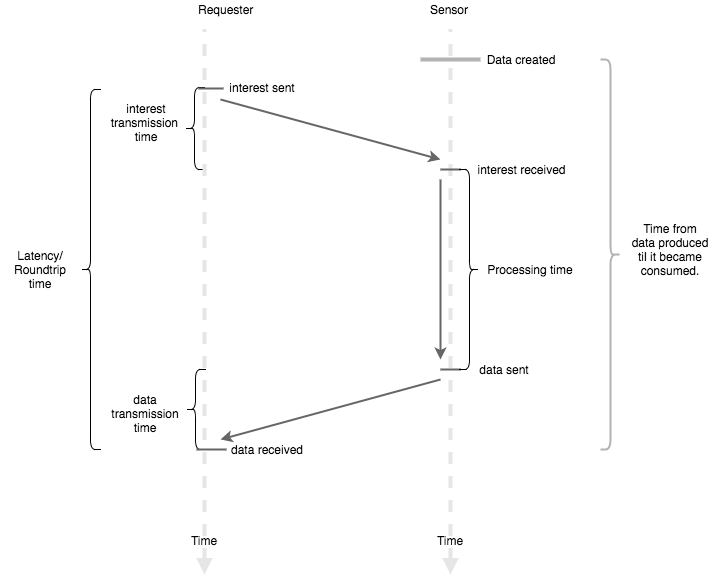
\includegraphics[width=\textwidth]{figures/latency.png}
    %\caption{Star topology structure on the left, Peer-to-peer on the right. write where it is taken from?}
    \caption{The roundtrip measurement is the time it takes for a client to initiate a request, and get data as a response. Transmission time is the time the bits spent on the wire or radio. Processing time is calculated from the time an interest was received til it was sent back to the requestor.}
    \label{fig:latency}
\end{figure}



\subsection{Result}
%\begin{itemize}
%\item How long does the roundtrip take for ping, peek.\\
% [When the debugging tool is turned on it will print out information (for instance if the interest object was found or not) on the terminal console. One reason to have two test, one with and without debugging turned on, is to validate that information is correct which can be done with debugging turned on. Another reason is to show how much processing power something as simple as printing can affect the overall latency]. 

The results from the latency times with ping6 are shown in figure \ref{fig:pingRTT}, where packet size, in bytes, sent on the radio link is shown on the x-axis and the latency time, in milliseconds, on the y-axis. The same axis layout holds for figure \ref{fig:peekwoutdbRTT} and \ref{fig:peekwdbRTT}, but those figures shows the roundtrip time for CCN peek in two different cases. One is with the essential information printed out on the debugging console. The other one does not print anything on the debugging console. \\\\
The results, illustrade in figure \ref{fig:pingRTT}, show that the median latency for a ping6 request is very close to around 25 ms from 93 bytes in packet size up to 123 bytes. The median latency when sending a CCN peek request without debugging, shown in figure \ref{fig:peekwoutdbRTT} is little above 25 ms for packet sizes the fragmentation limit. Roundtrip times when debugging is turned on, illustrated in figure \ref{fig:peekwdbRTT}, show a median of around 50 ms. The 20-25 ms difference (around 100$\%$) between the two peek results shows that there is a lot that can slow down the processing power, in this particular case it is only due to printing out massive amount of information toward the user in the terminal.\\\\
When the experiments started, the measurements showed that the round trip times was around 130 ms in median values. Those latencies was considered very high and unrealistic. It resulted in an investigation regarding where the processing time was spent on the sensor. Several timing checkpoints was set out and it showed later that there was code that put the sensor in sleep mode for 100 ms every time the sensor retrieved an \textit{interest}. It also revield several flaws in the CCN-lite portation that needed to be handled. When they were fixed, the result was a more optimal code base and better performing latency values which is shown in the previous paragraph.\\\\
%\item The difference in time. Point that it much conclude that the proccessing time of CCN is the bottleneck.\\
%The peek (from now only regarded without debugging) latency time is steady 90 ms slower compared to the ping counterpart. This indicates that most time differences between them must lay in the overhead it takes to process an incoming peek request for a sensornode. This makes sense when considering the differences between ping and peek, where ping responds as soon as possible, peek has to look up the content, process it and then respond toward the requester.
The CCN peek (from here on only concerning without debugging) latency time is only a few milliseconds apart from the ping counterpart when the same amount of data sent of the network. This indicates that, in a bigger perspective, the time it takes to process an incoming CCN interest is almost negligible for the sensornode although it is constrained. Although the difference is very small, when comparing latencies in figure \ref{fig:pingRTT} and figure \ref{fig:peekwoutdbRTT} one can see the small jump between them. This makes sense when considering that peek has to look up the content, process it and then respond to the requester, whereas ping would more or less respond direclty. 
The time resolution on the sensor equals to 1/128th second, equvivalent to 7.8 ms. Unforturnately, this makes it impossible to further investigate in the details of where the processing time is spent on the sensor. The couple of milliseconds in difference between a CCN peek and ping is not enough for the time resolution.
%\item The similarities regarding the curves flatness \\
\\\\
In all tests, the latency remain relativly flat even though the packet size is increasing, except the region around 123 byte to 128 byte. This indicates that the transmission delay has small to none overall effect on the latency. It also corresponds well to the fact that it theoretically takes 0.5 ms to send 127 bytes on a link that has a transmission rate of 250 kbit/s.
%\item The min values. Do we really get the lowest values?\\
\\\\
The fifteen to twenty millisecond jump in latency from 123 byte to 128 byte can be seen in all tests and is due to the 127 byte MTU of 802.15.4 which result in packet fragmentation at 127 bytes. The latency remains stable even after the fragmentation limit, which makes sense considering the flatness of the latency described above.
\\\\
%All measurements show a five to ten ms difference between the minimum latency and the median latency. Even though there was only a couple of such minimum values per hundred latency iterations, they show that the latency could be improved. There has been attempts to find the reason why this glitch occurs but without any success[Continue?].
All measurements show a five to ten milliseconds difference between the minimium latency and the average/median latency. The histogram for the ping and peek latency measurements are illustrated in figure \ref{fig:histPing} and \ref{fig:histPeek}. They show the number of roundtrips, for application sizes of 17, 22 and 27 bytes, that can be categorised together and thereby see if there is any outliers that can be obmitted. Both histograms show that there is only a few such outliers and the absolute majority of the roundtrips lay around 24-28 ms. This inidicates that, even though the average and median latencies are close to each other, the median value is the correct way of measurement.










% Please add the following required packages to your document preamble:
% \usepackage{graphicx}
\begin{table}[]
\centering
\resizebox{\textwidth}{!}
{%
\begin{tabular}{|l|l|l|l|l|l|l|l|l|l|l|l|l|l}
\cline{1-13}
CCN Peek & 1 (17) & 6 (22) & 11 (27) & 16 (32) & 21 (37) & 26 (42) & 31 (47) & 36 (52) & 41 (57) & 46 (62) & 51 (67) & 56 (72) &  \\ \cline{1-13}
Ping     & 17     & 22     & 27      & 32      & 37      & 42      & 47      & 52      & 57      & 62      & 67      & 72      &  \\ \cline{1-13}
802.15.4 & 93     & 98     & 103     & 108     & 113     & 118     & 123     & 128     & 133     & 138     & 143     & 148     &  \\ \cline{1-13}
\end{tabular}
}
\caption{Row one shows the length of the named data in bytes, if the data is named ``sensor'' it is equal to six bytes. The number in the parenthethis show the size of the application, CCN header and length of named data included. Row two shows the data payload of a ping message, equivialent to the application data. Row three shows the total amount of data sent on the 802.15.4 radio toward the sensor node.}

\label{tab:packetSizes}
\end{table}




%%%%%%%%%%%%%%%%% PING
\begin{figure}
\centering
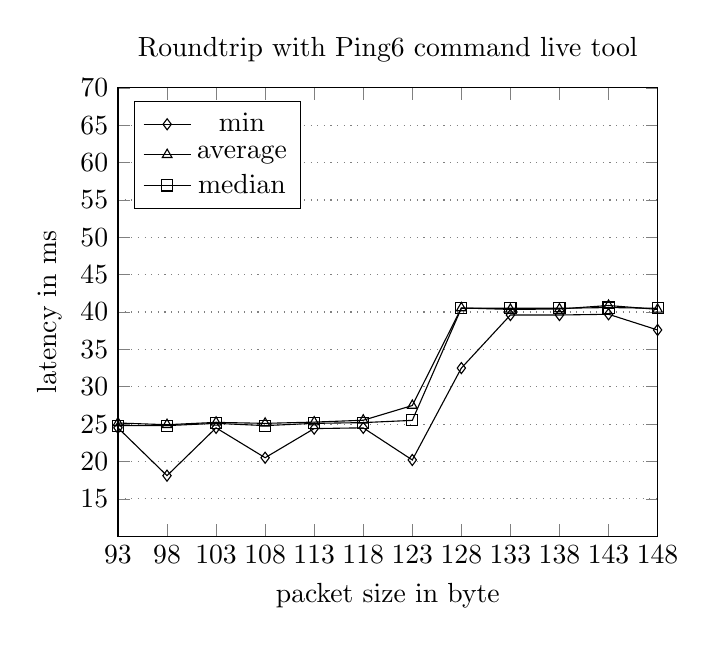
\begin{tikzpicture}
\begin{axis}[
    title={Roundtrip with Ping6 command live tool},
    xlabel={packet size in byte},
    ylabel={latency in ms},
    xmin=93, xmax=148,
    ymin=10, ymax=70,
    xtick={93,98,103,108,113,118,123,128,133,138,143,148,153},
    %xtick={17,22,27,32,42,47,52,57,62,67, 72, 77, 82},
    %ytick={20,40,60,80,100,120,140,160,180,200,220,240},
    ytick={15,20,25,30,35,40,45,50,55,60,65,70},
    legend pos=north west,
    grid style={dotted,gray},
    ymajorgrids=true,
]
\addplot[mark=diamond] coordinates {(93,24.5)(98,18.1)(103,24.5)(108,20.5)(113,24.4)(118,24.5)(123,20.2)(128,32.5)(133,39.6)(138,39.6)(143,39.7)(148,37.6)(153,39.7)};\addlegendentry{min}
\addplot[mark=triangle] coordinates {(93,25.148)(98,24.919)(103,25.232)(108,25.099)(113,25.269)(118,25.515)(123,27.486)(128,40.547)(133,40.349)(138,40.407)(143,40.873)(148,40.353)(153,40.789)};\addlegendentry{average}
\addplot[ mark=square] coordinates {(93,24.8)(98,24.8)(103,25.1)(108,24.8)(113,25.1)(118,25.2)(123,25.5)(128,40.5)(133,40.5)(138,40.5)(143,40.6)(148,40.5)(153,40.5)};\addlegendentry{median}

\end{axis}
\end{tikzpicture}
\caption{Latencies in milliseconds when pinging a sensornode with packet sizes from 93 byte to 148 byte transmitted over the radio. The latencies stays stable at around 27 ms up until 123 byte. After fragmentataion, the latency raise and stay stable at around 43 ms.}
%\caption{The difference between minimum, median and average values is neglectable between packet sizes of 108-123.}
%Latencies in milliseconds when pinging a sensornode with packet sizes from 93 byte to 153 byte transmitted over the radio. The latencies stays stable at around 27 ms up until 123 byte. After fragmentataion, the latency raise and stay stable at around 43 ms.
\label{fig:pingRTT}
\end{figure}

%%%%%%%%%%%%%%%%% WITHOUT DEBUG
\begin{figure}
\centering
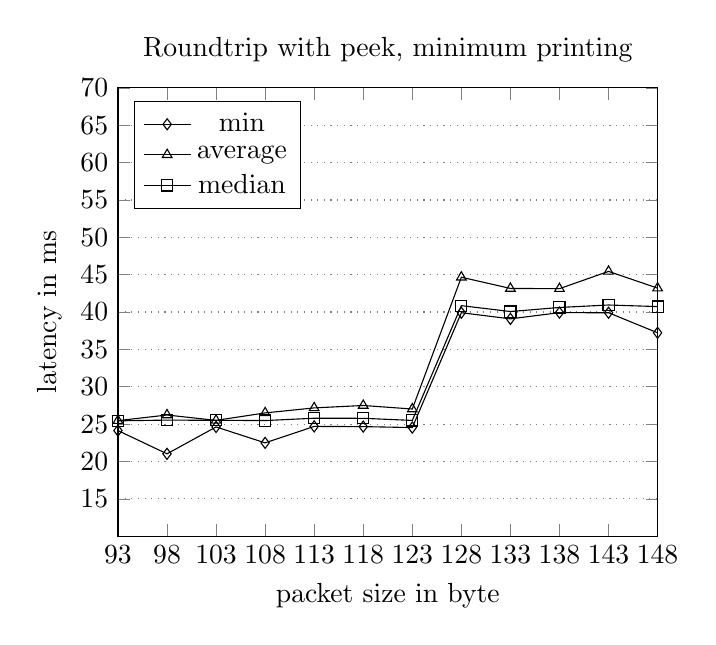
\begin{tikzpicture}
\begin{axis}[
    title={Roundtrip with peek, minimum printing},
    xlabel={packet size in byte},
    ylabel={latency in ms},
    xmin=93, xmax=148,
    ymin=10, ymax=70,
    xtick={93,98,103,108,113,118,123,128,133,138,143,148,153},
    %xtick={17,22,27,32,42,47,52,57,62,67, 72, 77, 82},
    %ytick={20,40,60,80,100,120,140,160,180,200,220,240},
    ytick={15,20,25,30,35,40,45,50,55,60,65,70},
    legend pos=north west,
    grid style={dotted,gray},
    ymajorgrids=true,
]
 
\addplot[ mark=diamond ] coordinates {(93,24.135)(98,21.021)(103,24.62)(108,22.488)(113,24.69)(118,24.663)(123,24.535)(128,39.908)(133,39.0863)(138,39.918)(143,39.904)(148,37.22)};\addlegendentry{min}
\addplot[ mark=triangle ] coordinates {(93,25.46426)(98,26.21715)(103,25.49883)(108,26.49811)(113,27.16887)(118,27.49096)(123,27.01817)(128,44.65865)(133,43.156053)(138,43.12575)(143,45.43817)(148,43.197726)};\addlegendentry{average}
\addplot[ mark=square ] coordinates {(93,25.439)(98,25.535)(103,25.5075)(108,25.4745)(113,25.7845)(118,25.775)(123,25.4915)(128,40.853)(133,40.06595)(138,40.61)(143,40.94)(148,40.7285)};\addlegendentry{median}


\end{axis}
\end{tikzpicture}
\caption{Latencies in milliseconds for peek interest requess of sizes from 93 byte to 148 byte. The latencies stays stable at around 123 ms between 93 byte to 123 byte. After fragmentation, the latency raise and stays stable at around 135 ms instead.}
\label{fig:peekwoutdbRTT}
\end{figure}
%Latencies in milliseconds for peek interest requests of sizes from 93 byte to 153 byte. The latencies stays stable at around 123 ms between 93 byte to 123 byte. After fragmentation, the latency raise and stays stable at around 135 ms instead.
%%%%%%%%%%%%%%%%% WITH DEBUG

\begin{figure}
\centering
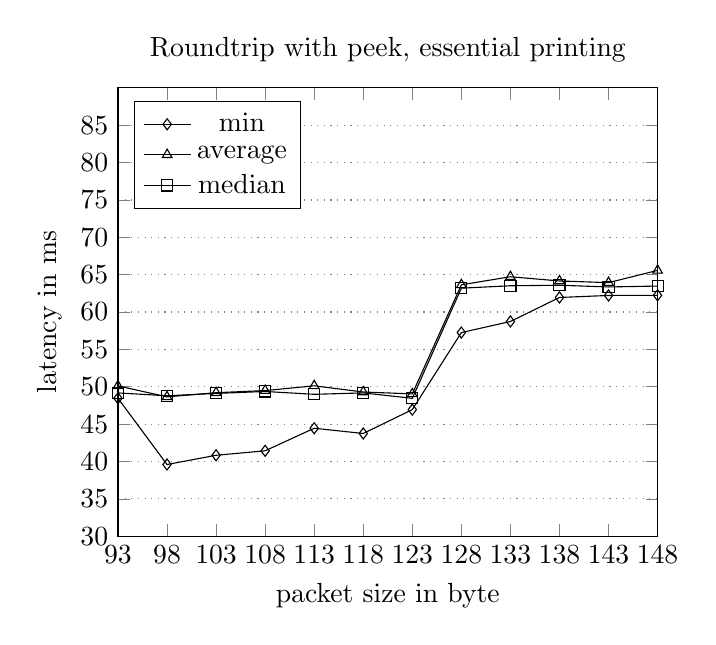
\begin{tikzpicture}
\begin{axis}[
    title={Roundtrip with peek, essential printing},
    xlabel={packet size in byte},
    ylabel={latency in ms},
    xmin=93, xmax=148,
    ymin=30, ymax=90,
    xtick={93,98,103,108,113,118,123,128,133,138,143,148},
    %xtick={17,22,27,32,42,47,52,57,62,67, 72, 77, 82},
    %ytick={20,40,60,80,100,120,140,160,180,200,220,240},
    ytick={15,20,25,30,35,40,45,50,55,60,65,70,75,80,85},
    legend pos=north west,
    grid style={dotted,gray},
    ymajorgrids=true,
]
 
\addplot[ mark=diamond ] coordinates {(93,48.463)(98,39.591)(103,40.828)(108,41.427)(113,44.445)(118,43.744)(123,46.936)(128,57.252)(133,58.734)(138,61.949)(143,62.218)(148,62.236)(153,61.883)};\addlegendentry{min}
\addplot[ mark=triangle ] coordinates {(93,50.11621)(98,48.64623)(103,49.20378)(108,49.48537)(113,50.12659)(118,49.29696)(123,49.0408)(128,63.64151)(133,64.72201)(138,64.15666)(143,63.9334)(148,65.57433)(153,64.98528)};\addlegendentry{average}
\addplot[ mark=square ] coordinates {(93,49.173)(98,48.791)(103,49.108)(108,49.3675)(113,48.987)(118,49.1745)(123,48.451)(128,63.1915)(133,63.516)(138,63.583)(143,63.3555)(148,63.475)(153,63.5055)};\addlegendentry{median}

\end{axis}
\end{tikzpicture}
\caption{Write same as with debugging, or is this graph necessary??}
\label{fig:peekwdbRTT}
\end{figure}



%%%%%%%%%%%%%%%%% PING SICS!!!!
%\begin{figure}
%\centering
%\begin{tikzpicture}
%\begin{axis}[
%    %title={Ping rtt-comparison},
%    xlabel={packet size in byte},
%    ylabel={latency in ms},
%    xmin=93, xmax=148,
%    ymin=10, ymax=70,
%    xtick={93,98,103,108,113,118,123,128,133,138,143,148,153},
%    %xtick={17,22,27,32,42,47,52,57,62,67, 72, 77, 82},
%    %ytick={20,40,60,80,100,120,140,160,180,200,220,240},
%    ytick={15,20,25,30,35,40,45,50,55,60,65,70},
%    legend pos=north west,
%    ymajorgrids=true,
%    grid style={dotted,gray},
%    ymajorgrids=true,
%]
%\addplot[ color=black, ] coordinates {(93,16.7)(98,18.2)(103,19.1)(108,25.6)(113,21.9)(118,20.4)(123,25.8)(128,%35.7)(133,34.0)(138,34.2)(143,37.9)(148,37.1)(153,41.1)};\addlegendentry{min}
%\addplot[ color=blue, ] coordinates {(93,25.653)(98,26.955)(103,26.982)(108,27.331)(113,27.283)(118,26.906)(123%,27.1)(128,42.548)(133,42.245)(138,42.368)(143,42.651)(148,43.245)(153,42.707)};\addlegendentry{average}
%\addplot[ color=red, ] coordinates {(93,26.8)(98,26.9)(103,27.1)(108,27.35)(113,27.3)(118,26.8)(123,27.1)(128,4%2.7)(133,42.5)(138,42.6)(143,42.8)(148,43.0)(153,42.6)};\addlegendentry{median}
%
%\end{axis}
%\end{tikzpicture}
%\caption{SICS BG!!}
%%\caption{The difference between minimum, median and average values is neglectable between packet sizes of %108-123.}
%%Latencies in milliseconds when pinging a sensornode with packet sizes from 93 byte to 153 byte transmitted %over the radio. The latencies stays stable at around 27 ms up until 123 byte. After fragmentataion, the %latency raise and stay stable at around 43 ms.
%\label{fig:scisrtt}
%\end{figure}


\begin{figure}
\centering
\pgfplotstableread[row sep=\\,col sep=&]{
    interval & 17byte & 22byte & 27byte \\
    <20       & 0  & 2  & 0 \\
    20--24    & 0  & 3  & 0  \\
    24--28    & 99 & 95 & 98 \\
    28<       & 1  & 0  & 2 \\
    }\mydata

\begin{tikzpicture}
    \begin{axis}[
            title={Histogram of ping measurements},
            ybar,
            bar width=0.6cm,%<- changed
            %width=\textwidth,
            width=12cm,
            %height=.9\textwidth,
            legend style={at={(0.2,1)},
                anchor=north,legend columns=-1},
            symbolic x coords={<20,20--24,24--28, 28<},
            xtick=data,
            nodes near coords,
            nodes near coords align={vertical},
            ymin=0,ymax=150,
            ytick={0,20,40,60,80,100},
            grid style={dotted,gray},
            ymajorgrids=true,
            height=5cm,
            ylabel={number of roundtrips},
            xlabel={time in ms},
            enlarge x limits={abs=2*\pgfplotbarwidth}
        ]
        \addplot [draw=black,fill=black!60] table[x=interval,y=17byte]{\mydata};
        \addplot [draw=black,fill=black!40] table[x=interval,y=22byte]{\mydata};
        \addplot [draw=black,fill=black!20] table[x=interval,y=27byte]{\mydata};
        \legend{17 , 22 , 27 }
    \end{axis}
\end{tikzpicture}
\caption{Histogram of ping latencies result. A majority of the roundtrips end up in the 24-28 ms span.}
\label{fig:histPing}
\end{figure}

\begin{figure}
\centering
\pgfplotstableread[row sep=\\,col sep=&]{
    interval & 17byte & 22byte & 27byte \\
    <20       & 0  & 0  & 0 \\
    20--24    & 0  & 2  & 0  \\
    24--28    & 100 & 91 & 99 \\
    28<       & 0  & 7  & 1 \\
    }\mydata

\begin{tikzpicture}
    \begin{axis}[
            title={Histogram of peek measurements with minimum printing},
            ybar,
            bar width=0.5cm,%<- changed
            width=12cm,
            %height=.9\textwidth,
            legend style={at={(0.2,1)},
                anchor=north,legend columns=-1},
            symbolic x coords={<20,20--24,24--28, 28<},
            xtick=data,
            nodes near coords,
            nodes near coords align={vertical},
            ymin=0,ymax=150,
            ytick={0,20,40,60,80,100},
            grid style={dotted,gray},
            ymajorgrids=true,
            height=5cm,
            ylabel={number of roundtrips},
            xlabel={time in ms},
            enlarge x limits={abs=2*\pgfplotbarwidth}
        ]
        \addplot [draw=black,fill=black!60] table[x=interval,y=17byte]{\mydata};
        \addplot [draw=black,fill=black!40] table[x=interval,y=22byte]{\mydata};
        \addplot [draw=black,fill=black!20] table[x=interval,y=27byte]{\mydata};
        \legend{17 , 22 , 27 }
    \end{axis}
\end{tikzpicture}
\caption{Histogram of CCN-peek latencies result. Almost all of the roundtrips ended up in the 24-28 ms interval.}
\label{fig:histPeek}
\end{figure}